\documentclass[12pt]{article}
\usepackage{amsmath,amssymb,amsthm}
\usepackage{xcolor,enumitem}
\usepackage{tikz}

\title{Section 5.1.3 – Strong Induction: Proving the Unprovable (Almost)}
\author{SWOSU Discrete Structures}
\date{}

\begin{document}
\maketitle

\section*{When Regular Induction Isn’t Enough}
Sometimes one domino can’t knock down the next — you need a running start!  
That’s where **strong induction** swoops in like a proof superhero.

Formally, if:
\[
\big( P(1)\wedge P(2)\wedge\dots\wedge P(k) \Rightarrow P(k+1) \big)
\]
then we can conclude \(P(n)\) is true for all \(n\ge1\).

\section*{Try It Yourself: Breaking Down Integers}
\textbf{Statement:} Every integer \(n>1\) can be written as a product of primes.

\begin{enumerate}[label=\alph*)]
\item \textbf{Base Case:} Prove it for \(n=2\). (Spoiler: it’s prime.)
\item \textbf{Inductive Hypothesis:}  
Assume all integers \(2,3,\dots,k\) can be written as products of primes.
\item \textbf{Inductive Step:}  
Show that \(k+1\) can also be written as a product of primes.
\item \textbf{Reflect:}  
Why do we need *strong* induction here instead of ordinary induction?
\end{enumerate}

\section*{Strong Induction in the Wild}
If you can climb any rung below you, not just the last one, you’ll always make it higher.  
This is how mathematicians prove things like:
\begin{itemize}
    \item Every amount of postage above 12¢ can be made with 4¢ and 5¢ stamps.
    \item Every integer greater than 1 has a prime factorization.
    \item Every coffee cup becomes a donut if you stretch it gently enough (okay, that’s topology, but still fun).
\end{itemize}

\begin{center}
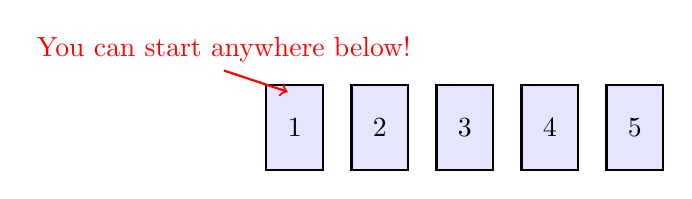
\begin{tikzpicture}[scale=0.9]
    \foreach \x in {1,...,5}{
        \draw[fill=blue!10,thick] (\x*1.2,0) rectangle ++(0.8,1.2);
        \node at (\x*1.2+0.4,0.6) {\x};
    }
    \node[red] at (0.6,1.7) {You can start anywhere below!};
    \draw[->,red,thick] (0.6,1.4) -- (1.5,1.1);
\end{tikzpicture}
\end{center}

\end{document}

